\documentclass[11pt]{article}
\usepackage[margin=1in]{geometry}
\usepackage{mathpazo}
\usepackage{amsmath,amssymb}
\usepackage{microtype}
\usepackage{booktabs}
\usepackage{graphicx}
\usepackage[dvipsnames]{xcolor}
\usepackage{tikz}
\usetikzlibrary{positioning,arrows.meta,calc,fit,backgrounds}
\usepackage[most]{tcolorbox}
\usepackage{enumitem}
\usepackage{listings}
\usepackage[font=small,labelfont=bf]{caption}
\usepackage{hyperref}
\hypersetup{colorlinks=true,linkcolor=MidnightBlue,citecolor=MidnightBlue,urlcolor=MidnightBlue}
\usepackage{cleveref}
\urlstyle{tt}
\def\UrlBreaks{\do\_\do/\do.}
\newcommand{\file}[1]{\nolinkurl{#1}}
\newcommand{\code}[1]{\texttt{#1}}
\newcommand{\mhh}{m_{hh}}
\newcommand{\bw}{\boldsymbol{\omega}}
\newcommand{\bp}{\boldsymbol{p}}
\newcommand{\bx}{\boldsymbol{x}}
\newcommand{\data}{\mathcal{D}}

\definecolor{trainable}{HTML}{1B6CA8}
\definecolor{physics}{HTML}{2E933C}
\definecolor{datac}{HTML}{7B4EA3}
\definecolor{warn}{HTML}{C0392B}

\newtcolorbox{keyidea}[1][]{enhanced,breakable,colback=physics!6,colframe=physics!70!black,
  fonttitle=\bfseries,title={#1},boxrule=0.6pt,arc=2pt,left=6pt,right=6pt}
\newtcolorbox{aside}[1][]{enhanced,breakable,colback=trainable!5,colframe=trainable!70!black,
  fonttitle=\bfseries,title={#1},boxrule=0.6pt,arc=2pt,left=6pt,right=6pt}
\newtcolorbox{assume}[1][]{enhanced,breakable,colback=datac!5,colframe=datac!70!black,
  fonttitle=\bfseries,title={#1},boxrule=0.6pt,arc=2pt,left=6pt,right=6pt}
\newtcolorbox{watch}[1][]{enhanced,breakable,colback=warn!5,colframe=warn!70!black,
  fonttitle=\bfseries,title={#1},boxrule=0.6pt,arc=2pt,left=6pt,right=6pt}
\setlist{itemsep=2pt,topsep=3pt}
\setlength{\emergencystretch}{3em}

\lstset{language=Python, basicstyle=\ttfamily\small, columns=fullflexible,
  keepspaces=true, commentstyle=\color{physics!70!black}\itshape,
  keywordstyle=\color{trainable!90!black}\bfseries, stringstyle=\color{datac},
  showstringspaces=false, frame=single, rulecolor=\color{gray!40},
  backgroundcolor=\color{gray!3}, xleftmargin=4pt, xrightmargin=4pt,
  aboveskip=6pt, belowskip=6pt}

\newcommand{\what}{\hat{\boldsymbol{\omega}}}

\title{\textbf{Why is the Bayesian network so confident?}\\[4pt]
\large Diagnosis and plan for a defensible Bayesian uncertainty for \texttt{HEFTNet}\\[4pt]
\normalsize For approval before any code is written}
\date{October 31, 2026}

\begin{document}
\maketitle

\begin{abstract}
\noindent
The full-data Bayesian network (\file{runs/BNN_poisson_full}) gives a posterior mean
almost as accurate as the fine-tuned ensemble, but a posterior standard deviation of only
0.5\% of the POWHEG noise, so that its pulls have a standard deviation of 1.37 just above
threshold. Before the Bayesian network appears in a paper, we must know \emph{why}. A
posterior that is too narrow can have four causes: (A) the chain has not explored the mode
it sits in, (B) it has not visited the other modes, (C) the likelihood claims the network
describes POWHEG better than it does, and (D) the prior. A and B are failures of the
computation; C and D are choices in the model. Only once all four are understood can we
say what Bayes' theorem actually delivers here. Evidence already in hand points strongly to
A, and the model-error study of the appendix shows that C is real. This plan proposes five
steps, cheapest first, each with a decision rule: a linearised Laplace approximation that
gives the within-mode width \emph{without sampling}; HMC with a dense mass matrix taken from
it; several chains from different starting points; a likelihood with a sampled model-error
term; and a prior-sensitivity check. Nothing is written until you approve; the decisions
are collected in \cref{sec:decisions}.
\end{abstract}

\begin{keyidea}[The message for the paper]
Bayes' theorem is not on trial. The posterior answers a precisely posed question: given
\emph{this} network, \emph{this} prior and a likelihood that says the POWHEG noise is the
only discrepancy, how well are the network's parameters, and hence its predictions,
determined? If the computation is done correctly, that answer is right, and if the
predictions are then too confident, the fault lies in the question, namely in the
likelihood, which ignores the error of the model itself. The plan is designed to end in one
of two defensible statements: either ``with an adequate sampler and a likelihood that
includes a model-error term, the Bayesian predictive uncertainty is calibrated and agrees
with the ensemble'', or a clear account of which of the four causes prevents this.
\end{keyidea}

\tableofcontents

% ===========================================================================
\section{What we observed}
\label{sec:observed}

\begin{table}[h]
\centering
\small
\begin{tabular}{lccc}
\toprule
 & median $s/\sigma_k$ & s.d.\ of pull, 255--555 GeV & s.d.\ of pull, $> 555$ GeV \\
\midrule
Bayesian network (\file{BNN_poisson_full}) & 0.005 & 1.37 & 1.06 \\
fine-tuned ensemble, bootstrap & 0.056 & 1.15 & 1.04 \\
\quad + model error, $a(m_{hh})$ & 0.32 & 1.02 & 1.00 \\
\bottomrule
\end{tabular}
\caption{Calibration on the 1,000 test spectra (from the draft appendix).}
\label{tab:obs}
\end{table}

The run: Gaussian likelihood with the known POWHEG variances (the \code{poisson} option),
hierarchical Gaussian prior with 16 Gibbs-sampled precisions \cite{Neal:1996}, warm start from
\file{runs/L1Loss}, 1,000 warm-up iterations, 1,000 samples, 800 leapfrog steps,
acceptance rate 0.72, final step size $\varepsilon \approx 7.7\times10^{-4}$. The effective
sample size of the two monitored predictions is about 135. The posterior mean differs from
the ensemble mean by a median of 0.8 ensemble standard deviations: a perfectly sensible
central value, with an implausibly narrow band around it.

% ===========================================================================
\section{Four ways a posterior can be too narrow}
\label{sec:four}

\begin{figure}[h]
\centering
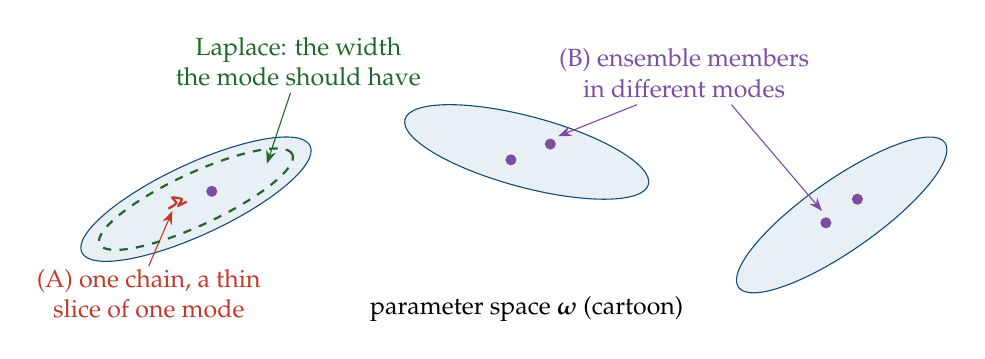
\begin{tikzpicture}[scale=1.0,>=Stealth]
  % modes
  \foreach \x/\y/\r in {0/0/25, 4.2/0.6/-15, 8.2/-0.2/35}{
    \fill[trainable!10] (\x,\y) ellipse [x radius=1.6, y radius=0.45, rotate=\r];
    \draw[trainable!70!black] (\x,\y) ellipse [x radius=1.6, y radius=0.45, rotate=\r];
  }
  % stuck chain in mode 1
  \draw[warn,thick] plot[smooth] coordinates {(-0.35,-0.12) (-0.25,-0.05) (-0.3,0.02) (-0.18,0.0) (-0.22,-0.08) (-0.12,-0.03)};
  \node[warn,font=\small,align=center] at (-0.6,-1.2) {(A) one chain, a thin\\slice of one mode};
  \draw[warn,->] (-0.6,-0.85) -- (-0.3,-0.15);
  % laplace ellipse
  \draw[physics!70!black,dashed,thick] (0,0) ellipse [x radius=1.35, y radius=0.33, rotate=25];
  \node[physics!70!black,font=\small,align=center] at (1.3,1.75) {Laplace: the width\\the mode should have};
  \draw[physics!70!black,->] (1.2,1.35) -- (0.9,0.45);
  % ensemble points
  \foreach \x/\y in {0.2/0.1, 4.0/0.5, 4.5/0.7, 8.0/-0.3, 8.4/0.0}{\fill[datac] (\x,\y) circle (2pt);}
  \node[datac,font=\small,align=center] at (6.2,1.6) {(B) ensemble members\\in different modes};
  \draw[datac,->] (5.6,1.2) -- (4.6,0.8);
  \draw[datac,->] (6.8,1.2) -- (7.95,-0.15);
  \node[font=\small] at (4.2,-1.4) {parameter space $\bw$ (cartoon)};
\end{tikzpicture}
\caption{Cartoon of the posterior: several separated modes (blue). A chain that mixes
poorly covers a thin slice of one mode (red); the linearised Laplace approximation gives the
width a well-sampled mode should have (green); ensemble members sit in different modes
(purple). Causes C and D change the shape of the ellipses themselves.}
\label{fig:cartoon}
\end{figure}

\begin{description}[leftmargin=1.2em]
  \item[A. Poor sampling within a mode.] HMC moves along stiff and soft directions alike
    with one step size, set by the stiffest. If the mass matrix does not equalise the
    curvatures, the soft directions are explored by a slow random walk, and a chain of
    $10^3$ iterations sees only a fraction of their width.
  \item[B. Modes not visited.] Networks have many separated modes (equally good solutions
    that are not related by a symmetry). A single chain stays in one
    \cite{Izmailov:2021}. The seeds ensemble
    shows that about 80\% of the ensemble variance is of this kind.
  \item[C. An over-confident likelihood.] The likelihood $\prod_k
    \mathcal{N}(t_k; f_k, \sigma_k^2)$ asserts that the network can represent the true
    cross section exactly and that the POWHEG noise is the only discrepancy. The model-error
    study says otherwise: on data not used in the training, a further variance
    $a\,\sigma_k^2$ with $a = 0.1$--0.75 is needed.
  \item[D. The prior.] With $2.7\times10^5$ training rows the likelihood dominates every
    direction that affects the predictions at points like the training points; the prior
    mainly controls the directions the data leave free, which hardly affect the predictions.
    A factor of ten from the prior would be surprising, but it is cheap to check.
\end{description}

\begin{watch}[A and B are different questions]
Even a perfect sampler need not make the posterior as wide as the ensemble. Whether the
modes of \cref{fig:cartoon} contribute to the posterior depends on their probability
\emph{mass}: if one mode has a mass $e^{100}$ times that of the others, the posterior is
that mode, and the ensemble spread, although a fair description of the variability of the
\emph{training procedure}, is not part of the Bayesian answer. Several chains tell us which
case we are in (\cref{sec:chains}).
\end{watch}

% ===========================================================================
\section{Evidence already in hand}
\label{sec:evidence}

\subsection{An identity: the effective number of parameters}

For a model linear in its parameters, $f = J\bw$, with Gaussian noise of known variances
$\sigma_k^2$ and a Gaussian prior of precision $A$, the posterior covariance is
$\Sigma = (J^{\mathsf T} W J + A)^{-1}$ with $W = \mathrm{diag}(1/\sigma_k^2)$, and
\begin{equation}
  \sum_{k=1}^{N} \frac{\mathrm{Var}_\text{post}[f_k]}{\sigma_k^2}
  = \mathrm{tr}\big(J^{\mathsf T} W J\, \Sigma\big)
  = \sum_i \frac{\lambda_i}{\lambda_i + \alpha_i} \equiv \gamma ,
  \label{eq:gamma}
\end{equation}
where, for a prior $A = \alpha I$, the $\lambda_i$ are the eigenvalues of
$J^{\mathsf T}WJ$. This is MacKay's ``number of well-determined parameters''
\cite{MacKay:1992}: each direction pinned down by the data contributes one, each direction
left to the prior contributes nothing, so $0 \le \gamma \le p$. Near a mode a network is
approximately linear in its parameters, so \cref{eq:gamma} applies approximately: the
sum over the training rows of $s_k^2/\sigma_k^2$, with $s_k$ the posterior standard
deviation of the prediction, counts the well-determined parameters.

\begin{keyidea}[What the run says]
Estimating the sum as $N$ times the average of $s_k^2/\sigma_k^2$ over the test spectra
(right panel of \cref{fig:evidence}), the Bayesian run gives $\gamma \approx 50$ out of
$p = 3{,}944$ parameters. For a network that represents 23 functions of $m_{hh}$ well
enough to give $\chi^2/N \approx 1.1$ on 80 bins over a 5-dimensional parameter space,
that is far too few. The fine-tuned ensembles, which are not posteriors, give 3,100--4,800:
the order of magnitude a well-determined network of this size should have. A correctly
sampled single mode is therefore expected to give a width of order the ensemble spread,
roughly ten times what the chain reports. This points to cause A.
\end{keyidea}

\begin{figure}[h]
\centering
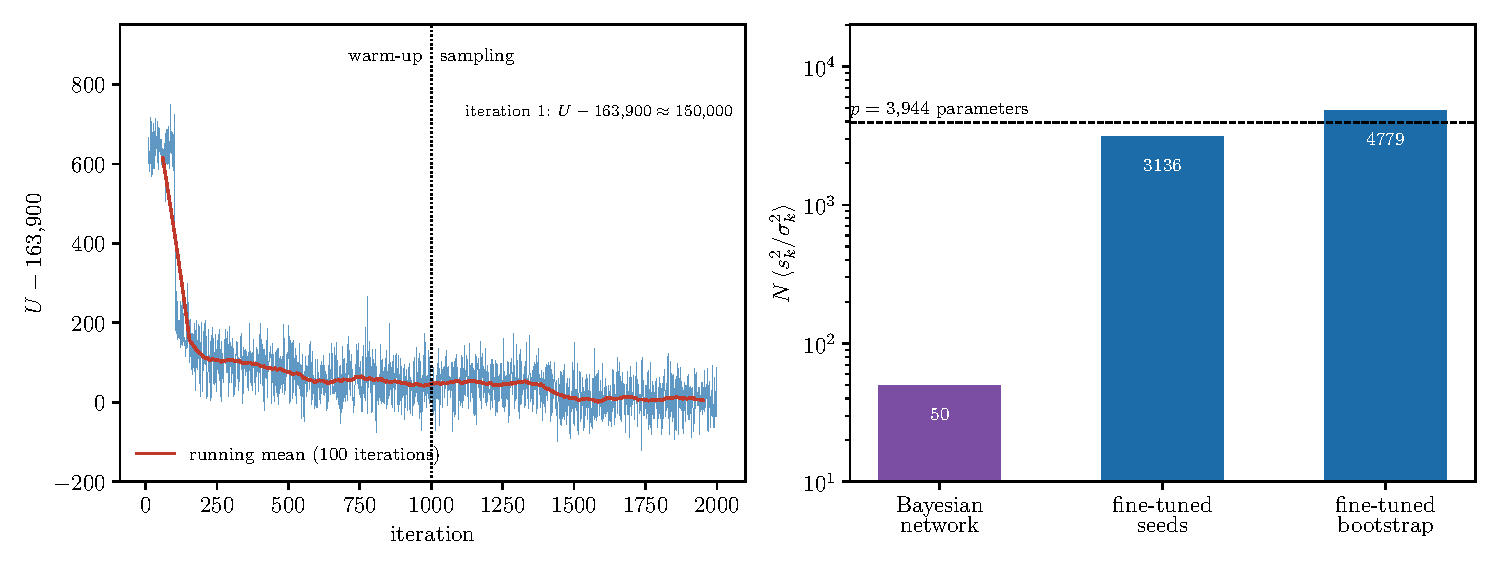
\includegraphics[width=\textwidth]{fig_evidence.pdf}
\caption{Left: the potential energy $U$ of \file{BNN_poisson_full} from iteration 10 on (it
starts 150,000 higher, at the L1 solution, and falls within ten iterations). It falls in
steps, at the first mass-matrix updates, and is still drifting downwards during sampling,
by about 100 over 1,800 iterations, two standard deviations of its fluctuations. Right:
$N\langle s_k^2/\sigma_k^2\rangle$, an estimate of the number of well-determined
parameters, \cref{eq:gamma}, for the Bayesian network and, for comparison, for the two
fine-tuned ensembles.}
\label{fig:evidence}
\end{figure}

\subsection{The chain was still relaxing}

The left panel of \cref{fig:evidence} shows that the chain reached the $\chi^2$ region
within ten iterations, sat nearly still for the first 150 iterations (the step size was
$\sim\!10^{-7}$ until the first mass-matrix updates), and has been drifting slowly
downhill ever since. A drift that persists through the whole sampling phase means the chain
has not reached its stationary distribution; samples drawn while it relaxes are too tightly
clustered. Note that the size of the fluctuations of $U$ (standard deviation 45, close to
$\sqrt{p/2} = 44$ expected for a $p$-dimensional Gaussian) is \emph{not} evidence of
good mixing: they are dominated by the stiff directions, which mix fast, and by the Gibbs
updates of the 16 precisions.

\subsection{The step size}

The leapfrog integrator is stable only if $\varepsilon \lesssim 2/\sqrt{\lambda_\text{max}}$,
where $\lambda_\text{max}$ is the largest curvature of $U$ in the coordinates set by the
mass matrix. If the diagonal mass matrix had equalised the curvatures, $\varepsilon$ would
be of order $p^{-1/4} \approx 0.1$ and a few tens of leapfrog steps would cross a mode. The
tuned $\varepsilon \approx 8\times10^{-4}$ implies a remaining curvature ratio of order
$10^6$: strong correlations between parameters, which a diagonal mass matrix cannot remove.
800 leapfrog steps then move the soft directions by only a fraction of their width per
iteration. There is a further trap: the mass matrix is estimated from the spread of the
chain during warm-up, so a direction that barely moves gets a small estimated variance and
moves even less in the next window.

\subsection{The likelihood is too confident}

At the end of the run, $U \approx 163{,}900$. The prior term
$\tfrac12\sum_i\tau_{g(i)}\omega_i^2$ is about $p/2 \approx 2{,}000$, the rest is the
likelihood term $\tfrac12\sum_k r_k^2$: $\chi^2 \approx 1.18$ per training row (with the
training variances, which include the one-event term and are therefore, if anything,
generous), where a correct
noise model with $\gamma \ll N$ well-determined parameters should give $1 - \gamma/N
\approx 1$. The training data themselves therefore say what the test spectra said: the
residual variance is about 20\% larger than the POWHEG noise, on average over $m_{hh}$
(cause C).

% ===========================================================================
\section{Step 1: the linearised Laplace approximation}
\label{sec:laplace}

\subsection{What it is}

Near a mode $\what$, replace the network by its linearisation
$f(\bx;\bw) \approx f(\bx;\what) + \boldsymbol{j}(\bx)^{\mathsf T}(\bw - \what)$, with
$\boldsymbol{j} = \partial f/\partial\bw$. The posterior is then Gaussian, with
precision (the generalised Gauss--Newton matrix plus the prior)
\begin{equation}
  H = \sum_{k=1}^{N} \frac{\boldsymbol{j}_k \boldsymbol{j}_k^{\mathsf T}}{\sigma_k^2}
    + \mathrm{diag}(\tau_{g(i)}) ,
  \label{eq:H}
\end{equation}
and the predictive standard deviation at any point is
\begin{equation}
  s(\bx) = \sqrt{\boldsymbol{j}(\bx)^{\mathsf T} H^{-1} \boldsymbol{j}(\bx)} .
  \label{eq:laplace_s}
\end{equation}
This is MacKay's original approach to Bayesian networks \cite{MacKay:1992}, revived in
recent years as the ``linearised Laplace'' or ``GLM predictive''
\cite{Immer:2021,Daxberger:2021}. It needs no sampling: one pass over the training rows to
build $H$, a Cholesky factorisation, and one pass over the points of interest.

\begin{aside}[Why it is cheap here]
$H$ is $3{,}944 \times 3{,}944$: 15.6 million numbers, 125~MB in double precision. Each
row's gradient $\boldsymbol{j}_k$ is obtained with \code{torch.func} (\code{vmap} of
\code{grad}) for a chunk of a few thousand rows at a time; the chunk's contribution
$J^{\mathsf T} W J$ is one matrix product. The 274,152 rows take of order a minute on the
5090; the Cholesky factorisation a second.
\end{aside}

\subsection{What it delivers}

\begin{enumerate}
  \item The within-mode width $s_k$ on the test spectra, to be compared with the chain's
    0.005$\,\sigma_k$ and the ensemble's 0.056$\,\sigma_k$.
  \item $\gamma = \mathrm{tr}(J^{\mathsf T}WJ\,H^{-1})$ exactly, \cref{eq:gamma}.
  \item The eigenvalues of $H$: its condition number tells us how badly a diagonal mass
    matrix must fail, and how long chains would have to be.
  \item The mass matrix for Step 2.
\end{enumerate}

\begin{assume}[Where to expand]
The expansion point should be a mode of the \emph{posterior}, i.e.\ a minimum of the
$\chi^2$ plus the prior. The fine-tune with $\delta = \infty$ (\file{runs/FT_chi2}, from
\file{code/heft_finetune.ipynb}; it is not in the Mac's \file{runs} folder, so it is
presumably on the 5090) is the $\chi^2$ minimum; a short polish with the prior term added (the fine-tune with a weight
penalty $\tfrac12\sum_i \tau_{g(i)}\omega_i^2$, using the precisions of the last
Bayesian sample) turns it into the posterior mode. We also expand about each of the 20
fine-tuned ensemble members ($\delta = 2$): this gives a \emph{mixture of Laplace
approximations} \cite{Eschenhagen:2021}, a cheap preview of Steps 2--3.
\end{assume}

\begin{keyidea}[Decision rule after Step 1]
\begin{itemize}
  \item Laplace width $\gg 0.005\,\sigma_k$ (we expect a few per cent of $\sigma_k$):
    cause A confirmed; go to Step 2.
  \item Laplace width $\approx 0.005\,\sigma_k$: the mode really is that narrow; the
    sampler is not the problem, and the answer must come from B and C (Steps 3--4).
\end{itemize}
\end{keyidea}

\begin{watch}[Limits of the approximation]
The Gauss--Newton matrix drops the term $\sum_k r_k\,\partial^2 f_k/\partial\bw^2$; with
$r_k$ of order the noise and the model near a mode, that term is small, and dropping it
keeps $H$ positive. The linearisation is only as good as the network is linear over the
width of the mode, which is exactly what Step 2 tests.
\end{watch}

% ===========================================================================
\section{Step 2: HMC with a dense mass matrix}
\label{sec:dense}

If the momenta are drawn with covariance $M = H$ (\cref{eq:H}), the Hamiltonian dynamics
see a posterior that is, near the mode, a unit sphere: all directions have the same
curvature, the step size can be of order $0.1$--$0.5$, and a trajectory of a few tens of
steps crosses the mode \cite{Neal:2011,Betancourt:2017}. Concretely, with the Cholesky
factor $H = LL^{\mathsf T}$:
\begin{equation}
  \bp = L\boldsymbol{z},\ \ \boldsymbol{z} \sim \mathcal{N}(0, I); \qquad
  K(\bp) = \tfrac12 \bp^{\mathsf T} H^{-1} \bp; \qquad
  \bw \leftarrow \bw + \varepsilon\, H^{-1}\bp ,
\end{equation}
where $H^{-1}\bp$ is two triangular solves with $L$. Each costs about $1.6\times10^7$
operations, negligible beside one gradient over 274,152 rows.

\begin{itemize}
  \item \textbf{Start} at the posterior mode of Step 1, not at the L1 solution: the warm-up
    then adapts the step size at equilibrium instead of during a descent.
  \item \textbf{Warm-up:} step size only (dual averaging); the dense mass matrix is fixed.
    Optionally recompute $H$ once at the end of warm-up, at the current point and with
    the current precisions $\tau_g$.
  \item \textbf{Leapfrog steps:} jittered around a trajectory length of order
    $\pi/2$ in the whitened units, i.e.\ $L \approx (\pi/2)/\varepsilon$; tens, not
    hundreds. Each iteration is therefore much cheaper than now, and chains can be much
    longer for the same GPU time.
  \item \textbf{The Gibbs updates of the $\tau_g$} change the prior part of the
    posterior's curvature; with the likelihood dominant this matters little, and the
    sampler stays correct for any fixed $M$, only its efficiency depends on it.
\end{itemize}

\begin{keyidea}[Success criteria for one chain]
No drift of $U$ in the sampling phase; within-chain width at the test points close to the
Laplace width; split-$\hat R < 1.01$ \cite{Vehtari:2021} and an effective sample size of several hundred for
predictions at many points (not two), and for $U$; ideally the same width whether the chain
starts at the mode or at a point displaced by a draw from the Laplace approximation.
\end{keyidea}

% ===========================================================================
\section{Step 3: several chains}
\label{sec:chains}

Run 4 to 8 chains, each with its own seed, started at the posterior modes polished from
different fine-tuned ensemble members (Step 1). The chains are independent processes
(separate \code{tmux} windows on the 5090, each with its own run folder); memory is not a
constraint. For each prediction we then have the within-chain variance $W$ and the
between-chain variance $B$.

\begin{itemize}
  \item \textbf{$\hat R$ on predictions} at a few thousand points: if $\hat R \gg 1$ the
    chains are in different modes, which no single chain will leave.
  \item \textbf{Do the modes matter?} Compare the chains' average $U$ and, more
    completely, their Laplace evidences
    $\ln Z_m \approx -U(\what_m) + \tfrac12 p \ln 2\pi - \tfrac12 \ln\det H_m$.
    Differences of order a few units: the modes carry comparable mass and the posterior
    is their mixture with roughly equal weights. Differences of tens to hundreds: the
    posterior is concentrated on the best mode(s).
  \item \textbf{Combining non-mixing chains.} Equal weights are correct only in the first
    case. Otherwise the chains are weighted by stacking, which chooses the weights that
    maximise the predictive density on held-out data \cite{Yao:2022}; the 38,076 unused
    training rows serve for that.
\end{itemize}

\begin{watch}[What this can and cannot establish]
If the mixture of chains reproduces the ensemble spread, the Bayesian and ensemble
uncertainties agree on the variability of the network. If the posterior is dominated by one
mode, the Bayesian answer is legitimately narrower than the ensemble: it then describes the
uncertainty of the best solution found, while the ensemble describes the variability of the
training procedure. Both are honest; they answer different questions, and the paper must
say which question each answers.
\end{watch}

% ===========================================================================
\section{Step 4: a likelihood that admits the model error}
\label{sec:modelerror}

Replace the noise variance by $(1 + a_r)\,\sigma_k^2$, where $r$ labels a few regions of
$m_{hh}$ (two, as in the appendix, or eight), and sample $a_r \ge 0$ along with the
network. Since the likelihood is Gaussian, the update of $s_r^2 = 1 + a_r$ is a conjugate
Gibbs step: with an inverse-Gamma prior IG$(\alpha_0,\beta_0)$,
\begin{equation}
  s_r^2 \sim \mathrm{IG}\Big(\alpha_0 + \tfrac12 N_r,\ \beta_0 + \tfrac12
  \sum_{k \in r} r_k^2\Big)\ \text{truncated to } s_r^2 \ge 1 ,
\end{equation}
where $N_r$ is the number of training rows in region $r$ and $r_k$ the pulls. The
machinery exists already (\code{GaussianLikelihood} samples one scale this way).

The Bayesian predictive distribution of the \emph{true} cross section in bin $k$ then has
variance $\mathrm{Var}_\text{post}[f_k] + a_r\sigma_k^2$, and that of a new POWHEG spectrum
adds $\sigma_k^2$; this is the Bayesian counterpart of the model-error term of the
appendix, learned from the training data. In addition, the posterior of the network itself
widens by $\sqrt{1 + a_r}$, since the data are now weighted less.

\begin{watch}[The independence assumption]
The term $a_r\sigma_k^2$ treats the model error as independent from bin to bin and from one
point $\theta$ to the next. It is not: the network's error is a smooth function, correlated
over neighbouring bins and parameter points. Treating it as independent overstates the
information in the data, so the sampled $a_r$ will be determined too precisely, and the
value learned from the training rows, to which the network has adapted, need not equal the
value needed on new data. (On average the two are similar: about 0.18 from the training
rows, \cref{sec:evidence}, and 0.09--0.29 from the held-out rows.) The principled remedy, a Gaussian-process
discrepancy term \cite{Kennedy:2001}, is beyond this project. We will compare the sampled
$a_r$ with the held-out values and, if they differ, say so and use the held-out
calibration, as in the appendix.
\end{watch}

% ===========================================================================
\section{Step 5: sensitivity to the prior}
\label{sec:prior}

With the Laplace machinery, the prior's influence on the width costs one Cholesky
factorisation per variant: change $\mathrm{diag}(\tau_g)$ in \cref{eq:H} and recompute
\cref{eq:laplace_s}. Variants: (i) the $\tau_g$ fixed at their posterior means; (ii) all
$\tau_g$ ten times smaller (a vaguer prior) and ten times larger; (iii) a different
grouping of the parameters. If the width at the test points changes by less than its
statistical uncertainty, cause D is excluded; only if it changes appreciably is a chain with
a modified prior worth running.

% ===========================================================================
\section{What could go in the paper}
\label{sec:paper}

\begin{table}[h]
\centering
\small
\begin{tabular}{p{0.38\textwidth}p{0.54\textwidth}}
\toprule
Outcome & Statement \\
\midrule
Laplace and dense-mass HMC agree; mixture of chains $\approx$ ensemble spread; with $a_r$
the pulls are calibrated &
``A Bayesian treatment, with a likelihood that includes a model-error term, gives
uncertainties consistent with the ensemble and calibrated on the test spectra.'' The
strongest outcome. \\
\addlinespace
As above, but one mode dominates &
``The posterior concentrates on one solution; its width describes that solution, while the
ensemble also captures the variability between solutions. Including the model error, both
are calibrated.'' \\
\addlinespace
Sampled $a_r$ smaller than the held-out values &
As above, with the held-out calibration of the model error, and a sentence on correlated
model errors \cite{Kennedy:2001}. \\
\addlinespace
None of the above converges &
Present the posterior mean only, as a cross-check of the central value, and state that a
converged posterior for $3{,}944$ parameters and $2.7\times10^5$ rows was beyond the
computing budget. \\
\bottomrule
\end{tabular}
\caption{Possible outcomes and the statement each supports.}
\end{table}

In every case the paper should report the diagnostics (effective sample sizes, $\hat R$,
the absence of drift), since a reader who has seen over-confident Bayesian networks before
will look for them first; and in no case should it present the current width of
$0.005\,\sigma_k$ as ``the Bayesian uncertainty''.

% ===========================================================================
\section{Code}
\label{sec:code}

\begin{itemize}
  \item \textbf{New module \file{dihiggs/laplace.py}}, heavily commented like the others:
\begin{lstlisting}
H = gauss_newton(model, X, V, prior_precision, chunk_size=4096)  # eq. (4)
chol = torch.linalg.cholesky(H)
s = predictive_sd(model, X_test, chol)                            # eq. (5)
gamma = effective_parameters(model, X, V, chol)                   # eq. (3)
lnZ = log_evidence(U_at_mode, chol)
\end{lstlisting}
  \item \textbf{\file{dihiggs/hmc.py}:} an option \code{mass='dense'} with
    \code{mass\_matrix=H} (Cholesky factor stored; momenta, kinetic energy and position
    update as in \cref{sec:dense}; warm-up adapts the step size only); checkpoints save the
    factor. The diagonal mode is unchanged. A model-error option for the
    \code{poisson} likelihood: \code{PoissonLikelihood(variance, regions=..., learn=True)},
    with the truncated inverse-Gamma Gibbs step.
  \item \textbf{New notebook \file{code/heft_laplace.ipynb}:} Step 1 and Step 5; writes
    \file{runs/LAPLACE/} with $H$, its eigenvalues, $\gamma$, the widths and, for each
    expansion point, the polished mode.
  \item \textbf{\file{code/heft_train_bnn.ipynb}:} new switches \code{START} (a parameters
    file, e.g.\ a polished mode), \code{MASS} (\code{'diag'} or \code{'dense'}),
    \code{MASS\_FILE}, \code{CHAIN} (an index that sets the seed and the run folder
    \file{runs/BNN_dense_chain<k>}), \code{MODEL\_ERROR\_REGIONS}.
  \item \textbf{New notebook \file{code/heft_bnn_chains.ipynb}:} combines the chains:
    $\hat R$, $W$ and $B$, evidences, stacking weights, and the calibration table and
    plots in the format of the appendix.
  \item \textbf{Toy test} in \file{code/hmc_toy.ipynb}: the dense mass matrix on a strongly
    correlated Gaussian, where the exact answer is known, before any real run.
\end{itemize}

% ===========================================================================
\section{Order of work}

\begin{enumerate}
  \item Step 1 and Step 5 (Laplace and prior sensitivity): minutes of GPU time; I can run
    them on the CPU here if you prefer, from the files in \file{runs/}. \emph{Gate:} the
    decision rule of \cref{sec:laplace}.
  \item Dense mass matrix in \file{hmc.py}, toy test, one chain from the polished mode.
    \emph{Gate:} the success criteria of \cref{sec:dense}.
  \item 4--8 chains (Step 3), then the same with the model-error term (Step 4).
  \item Write-up as \file{docs/bnn/bnn_run4.pdf}, and a revised Bayesian paragraph for the
    appendix.
\end{enumerate}

% ===========================================================================
\section{Decisions for you}
\label{sec:decisions}

\begin{keyidea}[Decisions before I proceed]
\begin{enumerate}
  \item \textbf{Laplace first, as a gate} before any new HMC code. Agreed?
  \item \textbf{Expansion points:} the posterior mode polished from \file{runs/FT_chi2},
    and modes polished from the 20 fine-tuned members of the bootstrap
    ensemble (on the Mac now \file{runs/ENS_bootstrap_huber_d2_1}). Agreed?
  \item \textbf{Dense mass matrix} from the Laplace $H$, fixed during warm-up (step size
    only), rather than a dense matrix estimated from the chain. Agreed?
  \item \textbf{Number of chains:} 4 or 8?
  \item \textbf{Model-error regions:} two (as in the appendix) or eight bands of $m_{hh}$?
  \item \textbf{Where Step 1 runs:} on the 5090 (a notebook you run) or here, on the CPU,
    with the parameter files I already have?
  \item \textbf{Location of this document:} \file{docs/bnn/bnn_plan2.pdf}?
\end{enumerate}
\end{keyidea}

\begin{thebibliography}{99}
\bibitem{MacKay:1992} D.~J.~C. MacKay, \emph{A practical Bayesian framework for
  backpropagation networks}, Neural Computation \textbf{4} (1992) 448.
\bibitem{Neal:1996} R.~M. Neal, \emph{Bayesian Learning for Neural Networks}, Lecture Notes
  in Statistics 118, Springer (1996).
\bibitem{Neal:2011} R.~M. Neal, \emph{MCMC using Hamiltonian dynamics}, in Handbook of
  Markov Chain Monte Carlo, Chapman \& Hall/CRC (2011), arXiv:1206.1901.
\bibitem{Betancourt:2017} M.~Betancourt, \emph{A conceptual introduction to Hamiltonian
  Monte Carlo}, arXiv:1701.02434.
\bibitem{Immer:2021} A.~Immer, M.~Korzepa and M.~Bauer, \emph{Improving predictions of
  Bayesian neural nets via local linearization}, AISTATS 2021, arXiv:2008.08400.
\bibitem{Daxberger:2021} E.~Daxberger et al., \emph{Laplace Redux: effortless Bayesian
  deep learning}, NeurIPS 2021, arXiv:2106.14806.
\bibitem{Eschenhagen:2021} R.~Eschenhagen et al., \emph{Mixtures of Laplace approximations
  for improved post-hoc uncertainty in deep learning}, NeurIPS 2021 Workshop on Bayesian
  Deep Learning, arXiv:2111.03577.
\bibitem{Izmailov:2021} P.~Izmailov, S.~Vikram, M.~D.~Hoffman and A.~G.~Wilson, \emph{What
  are Bayesian neural network posteriors really like?}, ICML 2021, arXiv:2104.14421.
\bibitem{Yao:2022} Y.~Yao, A.~Vehtari and A.~Gelman, \emph{Stacking for non-mixing Bayesian
  computations: the curse and blessing of multimodal posteriors}, JMLR \textbf{23} (2022) 1,
  arXiv:2006.12335.
\bibitem{Kennedy:2001} M.~C. Kennedy and A.~O'Hagan, \emph{Bayesian calibration of computer
  models}, J.~R.~Statist.\ Soc.~B \textbf{63} (2001) 425.
\bibitem{Vehtari:2021} A.~Vehtari, A.~Gelman, D.~Simpson, B.~Carpenter and
  P.-C.~B\"urkner, \emph{Rank-normalization, folding, and localization: an improved
  $\hat R$ for assessing convergence of MCMC}, Bayesian Analysis \textbf{16} (2021) 667.
\end{thebibliography}

\end{document}
